\documentclass[12pt]{article}
\usepackage{amssymb}
\usepackage[UTF8]{ctex}
\usepackage{geometry}
\usepackage{units}
\usepackage{pifont}
\geometry{
	a4paper,
	total={150mm,237mm},
	left=30mm,
	top=27mm,
	}
\usepackage{amsmath}
\usepackage{enumerate}
\usepackage{lipsum}
\usepackage{graphicx}
\usepackage{hyperref}
\usepackage{indentfirst}
\usepackage[graphicx]{realboxes}
\usepackage{booktabs}
\usepackage{cases}
\usepackage{subfig}  
\usepackage{float}

\setlength{\parindent}{2em}
\title{HW3}
\author{姓名:陈锐林,学号:21307130148}
\date{\today}

\begin{document}
\maketitle
\begin{LARGE}
    \noindent Chapter7\\
\end{LARGE}
\begin{large}
	\noindent Question1\\
\end{large}
\hspace*{2em}这题中三个任务用时相同,SJF和FIFO策略下,周转时间和响应时间是一样的。周转时间=(200+400+600)/3=400,而响应时间=(0+200+400)/3=200。-c验证后也确实如此。\\

\begin{large}
	\noindent Question2\\
\end{large}
\hspace*{2em}这题中三个任务用时不同,SJF和FIFO策略下,周转时间和响应时间可能会不一样,但是因为三个任务以100/200/300的顺序到达,于是两个策略的执行顺序仍是一样的。于是周转时间=(100+300+600)/3=333.3,而响应时间=(0+100+300)/3=133.3。-c验证后也确实如此。\\

\begin{large}
	\noindent Question3\\
\end{large}
\hspace*{2em}采用RR策略,显而易见地在响应时间上会有很大进步,为(0+1+2)/3=1;而周转时间会变大不少,为(598+599+600)/3=599。-c验证后也确实如此。\\

\begin{large}
	\noindent Question4\\
\end{large}
\hspace*{2em}根据前面几题和课本内容可以知道,要让SJF和FIFO策略的周转时间相同,工作负载需要满足:(1)工作不同时到达;(2)同时到达的工作需要以递增的方式排序(即FIFO策略近似为SJF策略调度后的任务序列)。\\

\begin{large}
	\noindent Question5\\
\end{large}
\hspace*{2em}若现在任务序列长度为{$a_1,a_2,a_3,\cdots,$}(递增)。对于SJF策略,响应时间就是{$0,a_1,a_1+a_2,\cdots,$},而对于RR策略,时间片为x,则响应时间为{$0,x,2x,3x,\cdots,$},那么要相同也就意味着每个任务的长度要等于RR的时间片。
\newpage
\begin{large}
	\noindent Question6\\
\end{large}
\hspace*{2em}根据SJF的安排,随着作业长度的增加,会导致后续任务的开始时间更晚;所以这题答案是响应时间会增加。而利用命令"python3 ./scheduler.py -p SJF -l 100,100,100 -c",安排三个相同长度的作业;从100-1000,取10次也能看出,响应时间从100递增到1000。\\

\begin{large}
	\noindent Question7\\
\end{large}
\hspace*{2em}设RR策略的时间片为T,共调度N个任务,假设任务长度 $\gg T$,那么平均响应时间就是(0+T+2T+$\cdots$+(N-1)T)/N=$\frac{n(n-1)}{2n}T$。\\

\begin{LARGE}
    \noindent Chapter8\\
\end{LARGE}
\begin{large}
	\noindent Question1\\
\end{large}
\hspace*{2em}根据题目的要求,两个工作/两个队列,限制作业长度和关闭IO。调用如下命令"python3 ./mlfq.py -n 2 -j 2 -m 15 -M 0 -s 50":两个任务长度分别是7和9。根据计算策略,先进行7再进行9,(两个队列时间片都是10);所以会得到响应时间为(0+7)/2=3.5,周转时间为(7+16)/2=11.5s。\\

\begin{large}
	\noindent Question2\\
\end{large}
\hspace*{2em}(1)Figure8.2:单个长工作的例子;可调用命令:"python3 ./mlfq.py -n 3 -l 0,200,0 -q 10 -c",该工作逐渐从最高优先级往下掉。\\
\hspace*{2em}(2)Figure8.3:即某个任务运行时,有新任务插入到最高优先级队列;可调用命令:"python3 ./mlfq.py -n 3 -q 10 -l 0,180,0:100,20,0 -c",时间片设为10,第一个任务0ms开始,需做180ms;第二个任务100ms加入,需做20ms。\\
\hspace*{2em}(3)Figure8.4:针对混合I/O密集型和CPU密集型,调用:"python3 ./mlfq.py -n 3 -Q 10,10,5 -l 0,175,0:50,25,1 -i 5 -S -c"。\\
\hspace*{2em}(4)Figure8.5:不采用优先级提升,调用:"python3  ./mlfq.py -n 3 -q 10 -l 0,120,0:100,50,5:100,50,5 -i 5 -S -c";采用优先级提示,调用"python3 ./mlfq.py -n 3 -q 10 -l 0,120,0:100,50,5:100,50,5 -i 5 -S -B 50 -c"。可以看到响应时间由1.67变为1.0;周转时间也降低1s左右。\\
\hspace*{2em}(5)Figure8.6:不采用愚弄反制时,调用"python3 ./mlfq.py -n 3 -q 10 -i 1 -S -l 0,200,0:80,100,9 -c";调用时去掉-S即可;从结果来看,不采取反愚弄机制会导致一个任务占据CPU过久。\\
\hspace*{2em}(6)Figure8.7:要体现优先级越低,时间片越长,可以调用:"python3 ./mlfq.py -n 3 -a 2 -Q 10,20,40 -l 0,200,0:0,200,0 -c",设置时间片为10/20/40,从时间片为10的最高优先级队列开始执行。
\newpage
\begin{large}
	\noindent Question3\\
\end{large}
\hspace*{2em}根据题目要求,要达到轮转调度类似的效果,应该满足:$T\leq\frac{maxL}{numJ}$,其中T是时间片大小;maxL是任务的最大长度;numJ是任务数。\\

\begin{large}
	\noindent Question4\\
\end{large}
\hspace*{2em}调用如下命令:"python3 ./mlfq.py -n 3 -l 0,200,0:50,99,9 -i 1 -S -c"。这样能得到三个队列,时间片都是10;io时间为1;第一个任务0ms开始,需做200ms,ioFreq为0;第二个任务50ms开始,需要使用99ms,ioFreq为9。
于是在这条命令下,总执行299s,在100s多的阶段,会出现第二个任务长时间占据CPU的情况。\\

\begin{large}
	\noindent Question5\\
\end{large}
\hspace*{2em}为了保证能占据至少5\%的CPU,在时间片为10ms的情况下,应该让提升的时间间隔在10/5\%,即200ms之内提升一次,让该任务提高到最高优先级,并且得到执行。考虑到其他任务的影响,应该在200ms以内更好。\\

\begin{large}
	\noindent Question6\\
\end{large}
\hspace*{2em}这题是探究完成I/O的作业插入在队列哪个位置对最后执行时间的影响。我们可以用接下来两条代码简单模拟:"python3 ./mlfq.py -n 2 -q 10 -l 0,50,0:0,50,11 -i 1 -S -c"和 "python3 ./mlfq.py -n 2 -q 10 -l 0,50,0:0,50,11 -i 1 -S -I -c"。第一条代码意为iobump=False,即I/O返回后并不会马上执行该任务;而第二条代码加上了-I标记,意为iobump=True,即I/O返回后马上执行。
于是分析结果我们会发现,用到I/O的任务在周转时间上得到了提升;但是在这个例子中整体的效率在下降(大大减缓了另一个任务的完成)。\\

\begin{large}
	\noindent 以下是一些运行截图:
\end{large}
\begin{figure}[h]
	\centering
	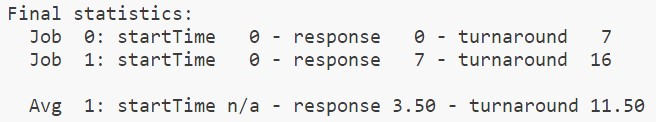
\includegraphics[height=3cm,width=10cm]{p1.jpg}
	\caption{Question1}
\end{figure}
\newpage
\begin{figure}[h]
	\centering
	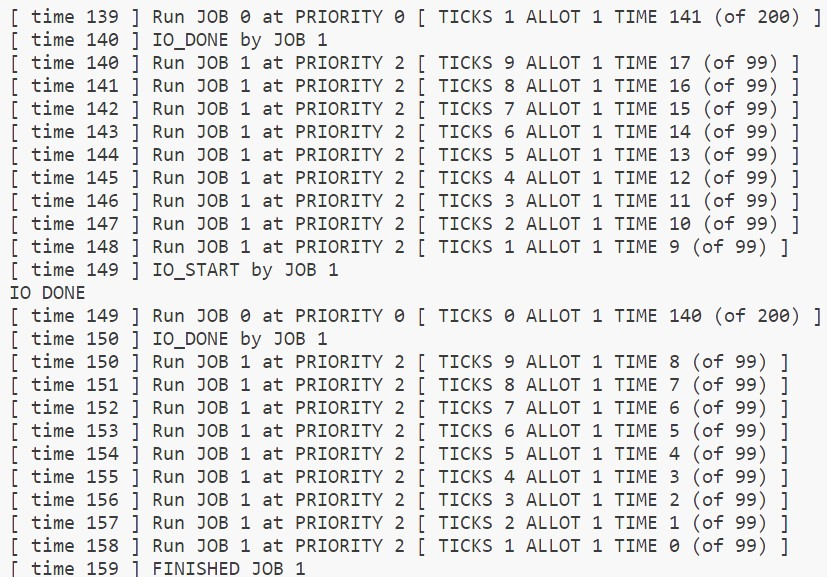
\includegraphics[height=10cm,width=10cm]{p4.jpg}
	\caption{Question4-任务1长时间占用CPU}
\end{figure}
\begin{figure*}[!h]
    \centering
    \subfloat[无-I]{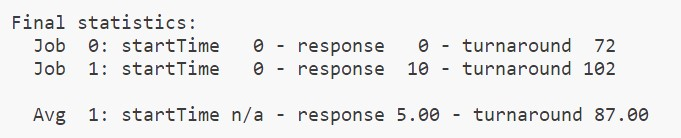
\includegraphics[width=7cm,height=2cm]{p3.jpg} \label{X}}
    \hfill
    \subfloat[有-I]{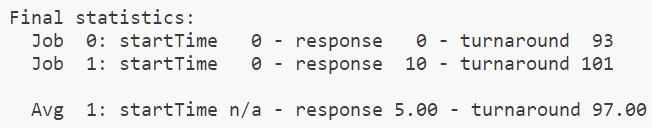
\includegraphics[width=7cm,height=2cm]{p2.jpg} \label{Y}}
	\caption{Question6}
\end{figure*}
\end{document}
